\chapter{System with uncertainties}
\label{cha:position_tip_uncertanties}

In the last part of our analysis we developed different control schemes to control the position of the tip when the arm had different values of inertia. As we already developed a model for the system in the nominal condition, we can design a control which considers the uncertainties of the parameters in the model and is still able to grant similar performances, and most importantly stability, for all the different system conditions.

In details we are changing the position of the tip of the arm and its value of inertia as expressed in the table below. The inertia is calculated in the same way as in paragraph \ref{sec: param est}.

\begin{table}[h!]
    \centering
    \begin{tabular}{||c c||} 
    \hline
    d[cm] & $J_L[Kgm^2]$ \\ 
    \hline\hline
    20 &  0.0032  \\ 
    \hline
    37 & 0.0062 \\
    \hline
    \end{tabular}
\end{table}

Whereas below we can see the A matrices in continuous time in both cases:

\[
A_{nominal} =
\begin{bmatrix}
    0  &  1.0377    &   -0.6104 &   -7.4061e-5       \\
    0  &  -37.199    &   603.06 &   0.2717       \\
    0  &  -0.0377    &   0.9948 &   1.0001       \\
    0  &  37.201    &   -987.46 &   -0.4496      
\end{bmatrix}   \]
\\
\[
A_{maxInertia} = 
\begin{bmatrix}
    0  &  1.0377    &   -0.6104 &   -7.4053e-5       \\
    0  &  -37.199    &   603.05 &   0.2717       \\
    0  &  -0.0377    &   0.9270 &   1.0001       \\
    0  &  37.201    &   -919.71 &   -0.4183        
\end{bmatrix} 
\]

\section{Robustness of State Space Control}

Knowing that the LQR control has robustness properties, we tried to apply the same control scheme we developed before to the system with different inertia parameters, as it is more reliable than the pole placement controller. 
As the observer relies on a correct model of the system, we decided to slow down the controller to better ensure stability of the closed loop system. 

In the plots below we can see the step response of the system with the maximum possible value of inertia in both cases, $\tau = 10$ and $\tau = 17$.

\begin{figure}[H]
     \centering
     \begin{subfigure}{0.47\textwidth}
         \centering
         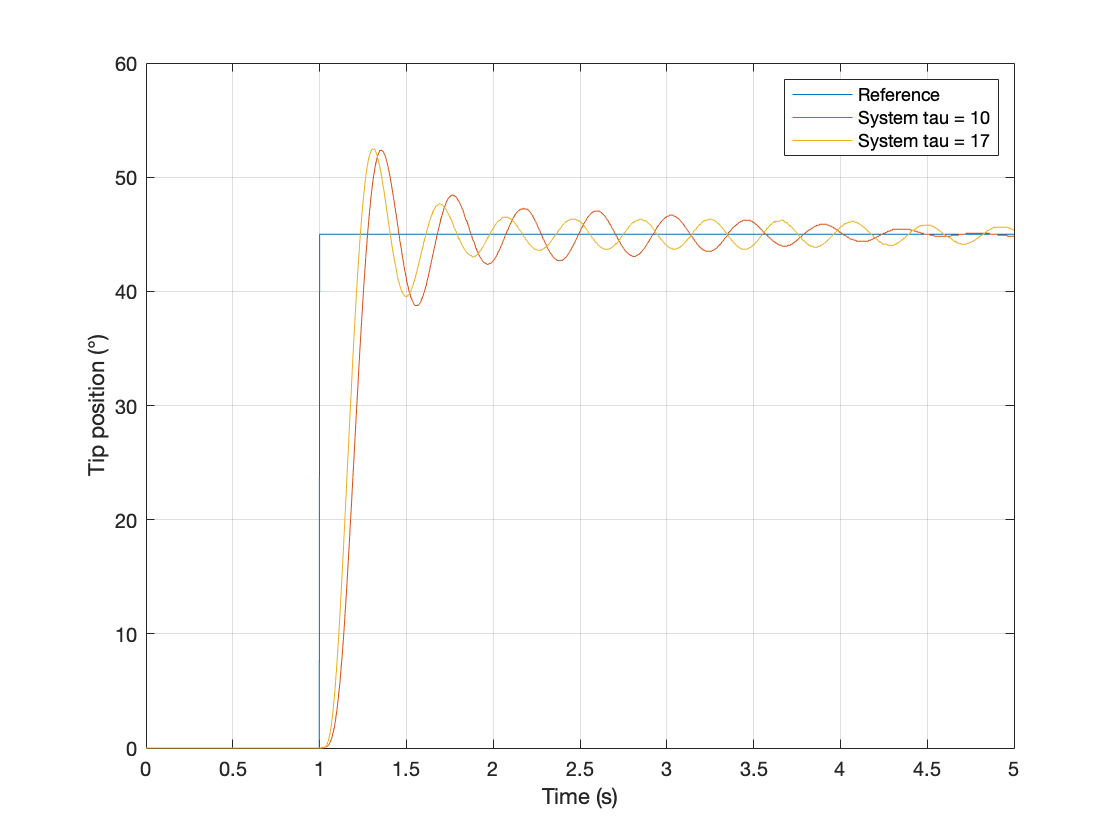
\includegraphics[width=\textwidth]{./images/Chapter 5/LQR/Step_unc.png}
     \end{subfigure}
     \hfill
     \begin{subfigure}{0.47\textwidth}
         \centering
         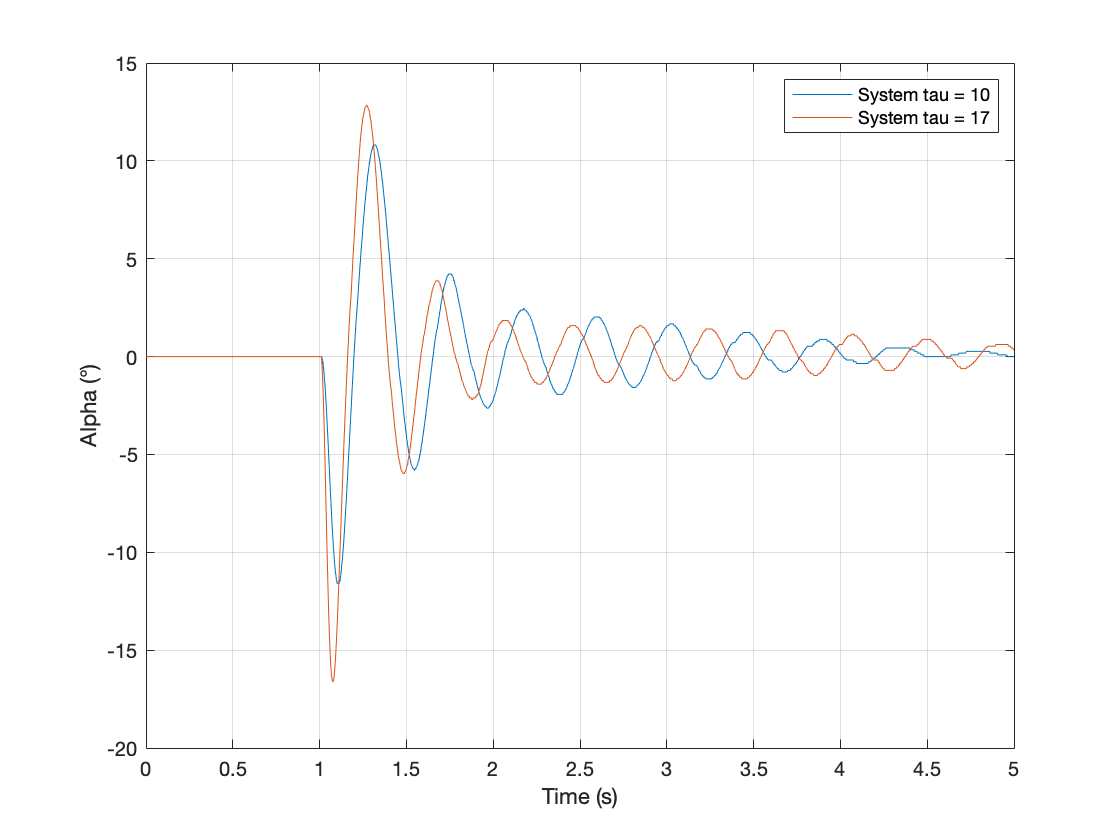
\includegraphics[width=\textwidth]{./images/Chapter 5/LQR/Alpha_unc.png}
     \end{subfigure}
\end{figure}

In the controller design we are not including the uncertainties related to the new system, so we cannot guarantee the same performances as in the nominal case, but still the system is able to reach the reference, although with oscillations.

\section{Robust control}

If we want to consider uncertainties of the model in our design we have to resort to robust control, which means the offline development of a controller that is able to maintain the same performances of the closed loop system even if the model of the system upon which it is designed is not reliable.

\subsection{$H_\infty$ control}

$H_\infty$ control is a type of optimal control scheme which grants robustness if the modeled plant presents uncertainties.

In the image below we can see how the design of the controller is done:

 \image[0.3]{./images/Chapter 5/H_inf/H-infty.png} 

 Where w is the array of exogenous inputs, z is the array of optimization variables, u and v are respectively the inputs and outputs of the enlarged system P and K is the $H_\infty$ controller. 

 In our case w is the reference signal and z is the difference between the reference and the tip position.
 As there was only one value to optimize, the introduction of weights was not necessary in this case.

 The obtained K, which is a 2x1 array of transfer functions, is then implemented as follows:

  \image[1]{./images/Chapter 5/H_inf/Control scheme.png}

Up until now we have a somewhat robust controller for our scheme which works perfectly fine on the nominal system, if we want to also take into consideration the information regarding the uncertainties in the model parameters, then we have to resort to $\mu$ synthesis control.

\subsection{$\mu$ synthesis control}

This kind of control is a generalization of $H_\infty$, the premises and the control scheme are identical but here we can also define a degree of uncertainty for our system, so after applying the controller, the robustness will be the one prescribed.

By looking at the A matrices for the tip position in the maximum inertia case at the beginning of the chapter, we can see that the elements $A(3,3), A(4,3)$ and $A(4,4)$ differ from the nominal case of $\approx 7\%$.

Knowing this information we defined an "uncertain state space" in Matlab having as nominal value the model we found previously and we put an $8\%$ uncertainty on those three parameters inside the A matrix. The $\mu$ synthesis function finds the controller $K_\mu$ by applying the $H_\infty$ algorithm recursively for each value of the parameter inside the specified range and keeping the best one.  

The obtained controller is thus:

\begin{equation*}
    K_\mu= \begin{bmatrix}
        \frac{-362.8 s^3-1.381e4 s^2 - 3.856 e5 s - 5.643 e 6}{s^4 + 81.54 s^3 +3545s^2+7.229e4s+1.329e6}   &
        \frac{-22.8s^3-1019s^2-2.894e4s-4.135e5}{s^4 + 81.54 s^3 +3545s^2+7.229e4s+1.329e6}
    \end{bmatrix}
\end{equation*}

\subsection{Validation}

In the plot below we can see the step response of this new control scheme where the different lines are due to the different values of inertia of the arm. 

 \image[1]{./images/Chapter 5/H_inf/Step.png} 

 As we can see, by increasing the inertia of the system the overshoot increases as well, but still the system is stable and also the performances are roughly the same, regardless of the uncertainties with the nominal model. 

 Unfortunately, when collecting data one of the signal was not starting from 0°, as we can see in the plot, but the conclusions we got are not affected by it, in fact it perfectly behaves like the other signals.